\documentclass[11pt,a4paper]{article}

\usepackage[utf8]{inputenc}
\usepackage{parskip}
\usepackage{tabularx}
\usepackage{amsmath}
\usepackage{amssymb}
\usepackage{amsthm}
\usepackage{geometry}
\usepackage{booktabs}
\usepackage{centernot}
\usepackage{hyperref}
\usepackage{eufrak}
\usepackage{graphicx}
\graphicspath{{pics/}}
\geometry{a4paper, left=20mm, right=20mm, top=20mm, bottom=20mm}

\usepackage{fancyhdr}
\pagestyle{fancy}
\lhead{Anthony Catterwell}
\chead{\textsc{University of Edinburgh}}
\rhead{Operating Systems}

\title{Operating Systems Lecture Notes}
\author{Anthony Catterwell}

\begin{document}
\maketitle
\tableofcontents

\break{}

\section{Lecture 2: Operating System Structure}
\subsection{Architectural features affecting OS\emph{s}}

\begin{itemize}
    \item These features were built primarily to support OS\emph{s}:
        \begin{itemize}
            \item timer (clock) operationg
            \item synchronisation instructions
            \item memory protection
            \item I/O control operations
            \item interrupts and exceptions
            \item protected modes of operation (kernel vs.\ user mode)
            \item privileged instructions
            \item system calls (including software interrupts)
            \item virtualisation architectures
        \end{itemize}
    \item ASPLOS
\end{itemize}

\subsection{Privileged instructions}
\begin{itemize}
    \item Some instructions are restricted to the OS
        \begin{itemize}
            \item known as \emph{privileged} instructions
        \end{itemize}
    \item Only the OS can:
        \begin{itemize}
            \item directly access I/O devices
            \item manipulate memory state management (page table pointers, TLB loads, etc.)
            \item manipulate special \emph{mode bits} (interrupt priority level)
        \end{itemize}
    \item Restrictions provide safety and security
\end{itemize}

\subsection{OS protections}
\begin{itemize}
    \item So how does the process know if a privileged instruction should be executed?
        \begin{itemize}
            \item the architecture must support at least two modes of operation:
                kernel mode, and user mode
            \item mode is set by status bit in a protected processor register.
                \begin{itemize}
                    \item user programs execute in user mode
                    \item OS executes in kernel (privileged) mode (OS == kernel)
                \end{itemize}
            \item Privileged instructions can only be executed in kernel (privileged) mode
                \begin{itemize}
                    \item if code running in user mode attempts to execute a privileged instruction,
                        the illegal execution trap.
                \end{itemize}
        \end{itemize}
\end{itemize}

\subsection{Crossing protection boundaries}
\begin{itemize}
    \item So how do user programs do something privileged?
        \begin{itemize}
            \item e.g.\ how can you write to a disk if you can't execute any I/O instructions?
        \end{itemize}
    \item User programs must call on OS procedure --- that is to ask the OS to do it for them.
        \begin{itemize}
            \item OS defines a set of system calls
            \item User-mode program executes system call instruction
        \end{itemize}
    \item Syscall instruction
        \begin{itemize}
            \item like a protected procedure call
        \end{itemize}
\end{itemize}

\subsection{Syscall}
\begin{itemize}
    \item The syscall instruction \emph{atomically}:
        \begin{itemize}
            \item saves the current PC
            \item sets the execution mode to privileged
            \item sets the PC to a handler address
        \end{itemize}
    \item Similar to a procedure call
        \begin{itemize}
            \item Caller puts arguments in a place the callee expects (registers, or stack)
                \begin{itemize}
                    \item One of the args is a syscall number, indicating which OS function
                        to invoke
                \end{itemize}
            \item Callee (OS) saves caller's state (registers, other control states) so it can
                use the CPU
            \item OS function code runs
                \begin{itemize}
                    \item OS must verify caller's arguments (e.g.\ pointers)
                \end{itemize}
            \item OS returns using a special instruction
                \begin{itemize}
                    \item Automatically sets PC to return address and sets execution mode to user.
                \end{itemize}
        \end{itemize}
\end{itemize}

\begin{center}{}
    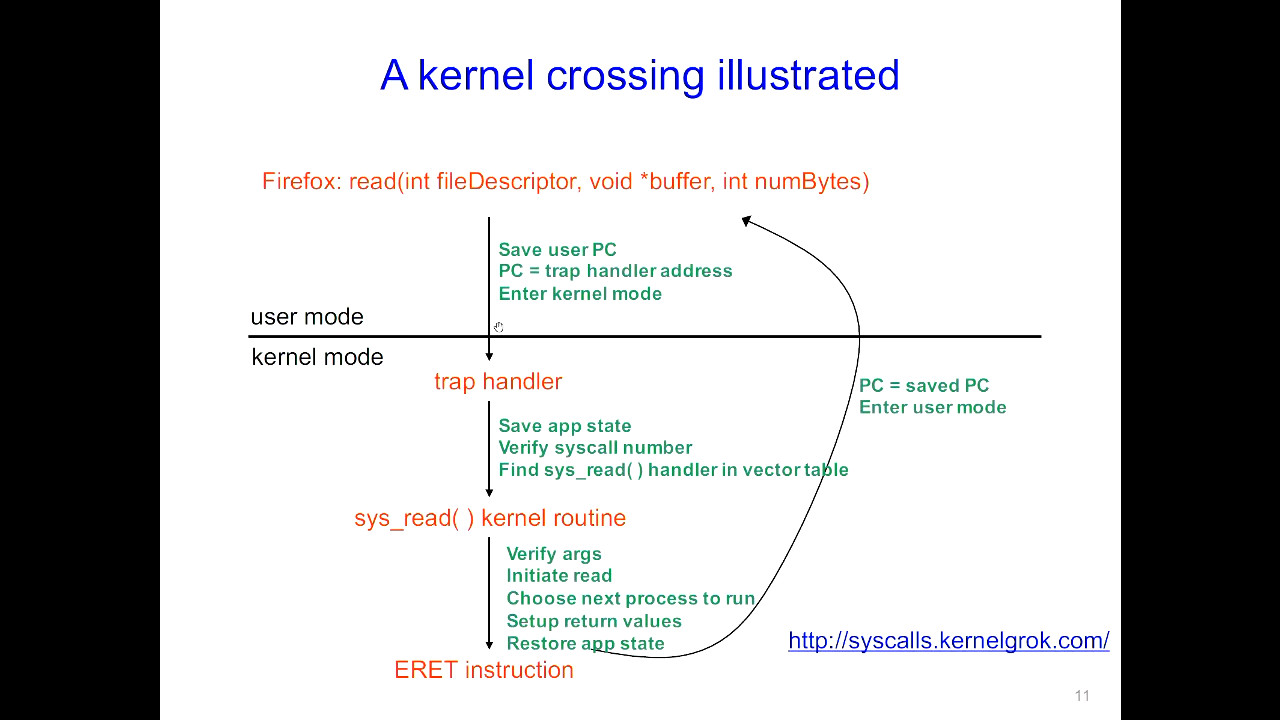
\includegraphics[height=270]{a_kernel_crossing_illustrated}
\end{center}

\subsection{System call issues}

\begin{itemize}
    \item A syscall is not a subroutine call, with the caller specifying the next PC.\
        \begin{itemize}
            \item the caller knows where the subroutines are located in memory;
                therefore they can be the target of an attack.
        \end{itemize}
    \item The kernel saves state?
        \begin{itemize}
            \item Prevents overwriting of values
        \end{itemize}
    \item The kernel verify arguments
        \begin{itemize}
            \item Prevents buggy code crashing the system
        \end{itemize}
    \item Referring to kernel objects as arguments
        \begin{itemize}
            \item Data copied between user buffer and kernel buffer.
        \end{itemize}
\end{itemize}

\subsection{Exception handling and protection}

\begin{itemize}
    \item \emph{All} entries to the OS occur via the mechanism just shown
        \begin{itemize}
            \item Acquiring privileged mode and branching to the trap handler are inseparable
        \end{itemize}
    \item Terminology
        \begin{itemize}
            \item \emph{Interrupt}: asynchronous; caused by an external device
            \item \emph{Exception}: synchronous; unexpected problem with instruction
            \item \emph{Trap}: synchronous; intended transition to OS due to an instruction
        \end{itemize}
        In all three cases, they are instances of where something strange happens,
        and the OS takes control: whether by accident, or by intention.
    \item Privileged instructions and resources are the basis for most everything:
        memory protection, protected I/O, limiting user resource consumption.
\end{itemize}

\subsection{OS structure}
\begin{itemize}
    \item The OS sits between application programs and the hardware
        \begin{itemize}
            \item it mediates access and abstracts away ugliness
            \item programs request services via traps or exceptions
            \item devices request attention via interrupts
        \end{itemize}
\end{itemize}

\subsection{Operating system design and implementation}

\begin{itemize}
    \item Design and implementation of OS not ``solvable'', but some approaches have proven
        successful.
    \item Internal structure of different OS\emph{s} can vary widely.
    \item Start the design by defining goals and specifications.
    \item Affected by choice of hardware, type of system.
    \item \emph{User} goals, and \emph{system} goals
        \begin{itemize}
            \item User goals: OS should be convenient to use, easy to learn, reliable, safe,
                and fast
            \item System goals: OS should be easy to design, implement, and maintain,
                as well as flexible, reliable, error-free, and efficient.
        \end{itemize}
    \item Important principle to separate
        \begin{itemize}
            \item \textbf{Policy}: \emph{What} will be done?
            \item \textbf{Mechanism}: \emph{How} to do it?
        \end{itemize}
    \item Mechanisms determine how to do something, policies decide what will be done.
    \item The separation of policy from mechanism is a very important principle,
        it allows maximum flexibility if policy decisions are to be changed later
        (e.g.\ timer).
    \item Specifying and designing an OS is a highly creative task of
        \emph{software engineering}.
\end{itemize}

\subsection{System layers}

\begin{center}{}
    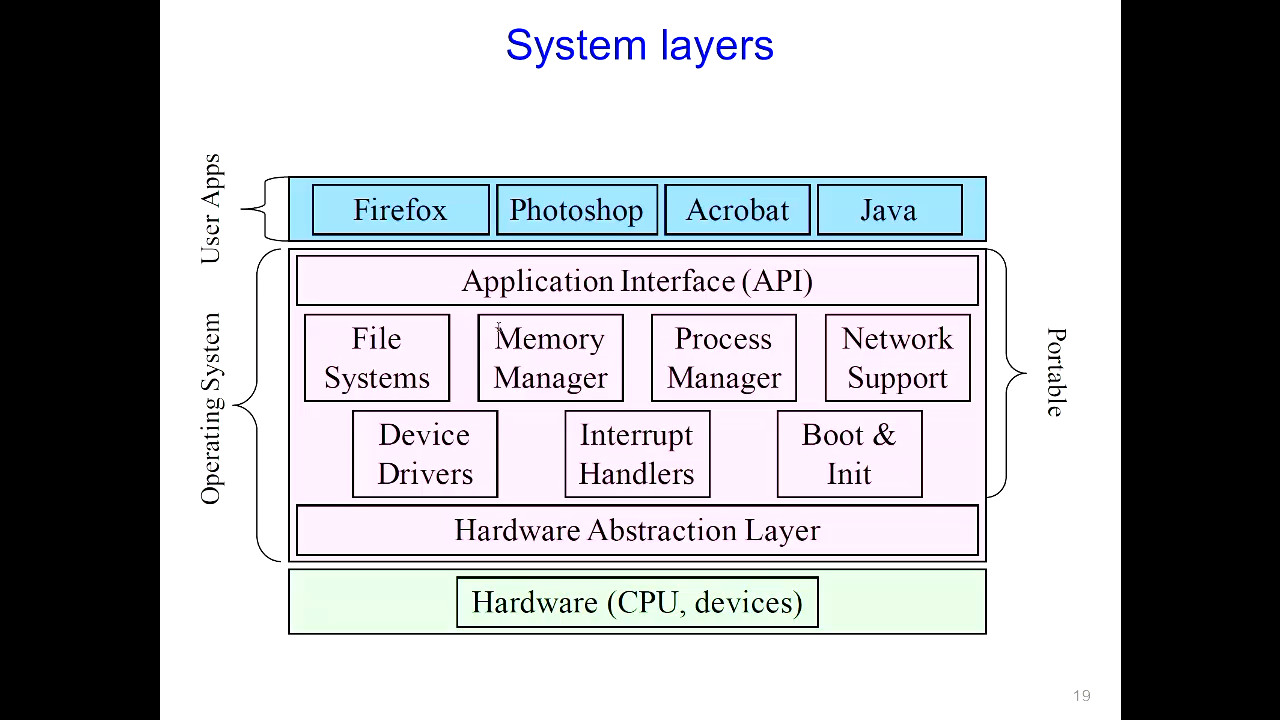
\includegraphics[height=280]{system-layers}
\end{center}

\subsection{Major OS components}
\begin{itemize}
    \item processes
    \item memory
    \item I/O
    \item secondary storage
    \item file systems
    \item protection
    \item shells
    \item GUI
    \item networking
\end{itemize}

\subsection{OS structure}

\begin{itemize}
    \item There's no clear hierarchy within an OS --- each of them needs access to different
        things.
    \item An OS consists of all these components, plus:
        \begin{itemize}
            \item many other components
            \item system programs (privileged, and non-privileged)
        \end{itemize}
    \item Major issue:
        \begin{itemize}
            \item how do we organize all this?
            \item what are all of the code modules, and where do they exist?
            \item how do they cooperate?
        \end{itemize}
    \item Massive software engineering and design problem
        \begin{itemize}
            \item design a large, complex program that:
                performs well, is reliable, is extensible, and is backwards compatible.
        \end{itemize}
\end{itemize}

\subsection{Monolithic design}
\begin{itemize}
    \item Traditionally, OS\emph{s} (like UNIX) were built as a \emph{monolithic} entity
        User programs | OS (everything) | hardware
    \item Major advantage: cost of module interactions is low (procedure call)
    \item Disadvantages:
        \begin{itemize}
            \item hard to understand
            \item hard to modify
            \item unreliable (no isolation between system modules)
            \item hard to maintain
        \end{itemize}
    \item What is the alternative? \\
        Find a way to organise the OS in order to simplify its design and implementation.
\end{itemize}

\subsection{Layering}

\begin{itemize}
    \item The traditional approach is layering
        \begin{itemize}
            \item implement OS as a set of layers
            \item each layer presents an enhanced \emph{virtual machine} to the layer above
        \end{itemize}
    \item The first description of this approach was Dijkstra's THE system
        \begin{itemize}
            \item Layer 5: \emph{Job managers} execute users' programs
            \item Layer 4: \emph{Device managers} handle devices and provide buffering
            \item Layer 3: \emph{Console manager} implements virtual consoles
            \item Layer 2: \emph{Page manager} implements virtual memories for each process
            \item Layer 1: \emph{Kernel} implements a virtual processor for each process
            \item Layer 0: \emph{Hardware}
        \end{itemize}
    \item Each layer can be tested and verified independently
    \item Imposes a hierarchical stricture
        \begin{itemize}
            \item but real systems are more complex:
                file systems require VM services (buffer);
                VM would like to use files for its backing store
            \item strict layering isn't flexible enough
        \end{itemize}
    \item Poor performance:
        each layer crossing has \emph{overhead} associated with it
    \item Disjunction between model and reality:
        systems modelled as layers, but not really built that way.
\end{itemize}

\subsection{Hardware abstraction layer}

\begin{itemize}
    \item An example of layering in modern operating systems
    \item Goal: separates hardware-specific routines from the \emph{core} OS
        \begin{itemize}
            \item Provides portability
            \item Improves readability
        \end{itemize}
\end{itemize}

\subsection{Microkernels}
\begin{itemize}
    \item Popular in the late 80s, early 90s
    \item Goal:
        minimize what happens in kernel;
        item organize rest of OS as user-level processes.
\item This results in:
    \begin{itemize}
        \item better reliability (isolation between components)
        \item easy of extension and customisation
        \item poor performance (user/kernel boundary crossings)
    \end{itemize}
\item First microkernel system was Hydra (CMU, 1970)
    \begin{itemize}
        \item Contemporaries: Mach (CMU), Chorus (French UNIX-like OS), OS X (Apple),
            in some ways NT (Microsoft)
    \end{itemize}
\end{itemize}

\begin{center}{}
    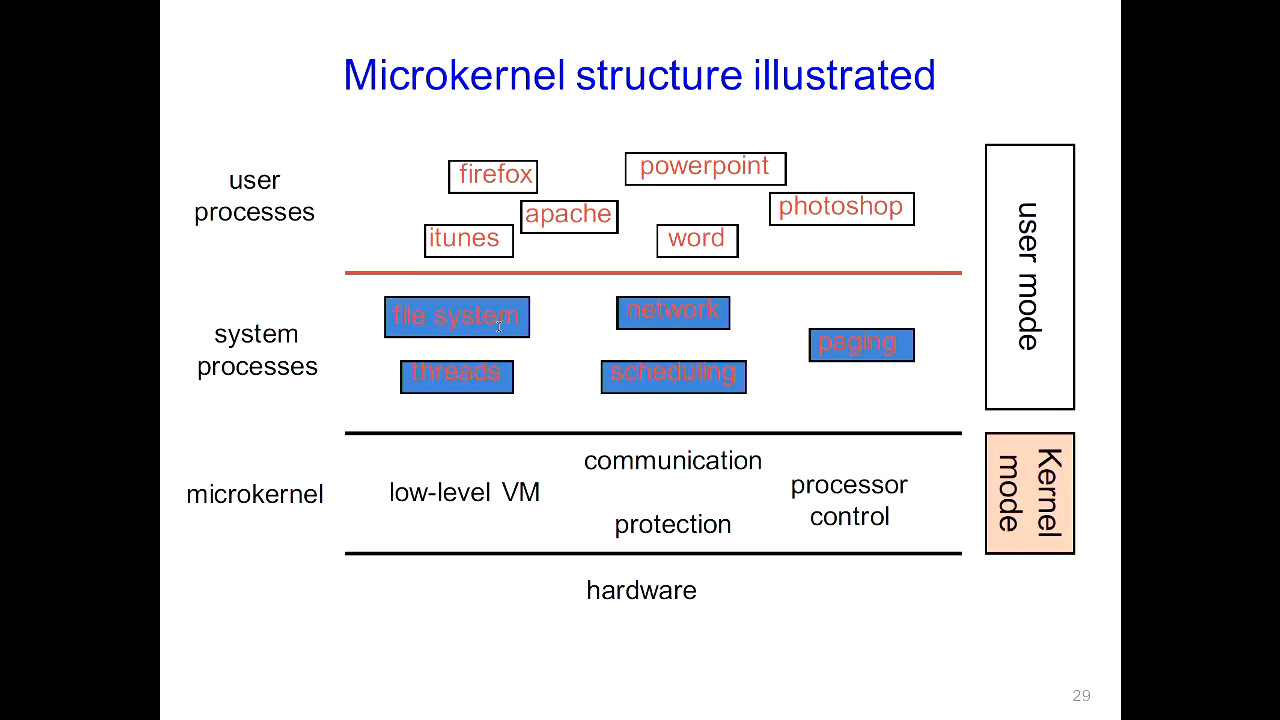
\includegraphics[height=270]{microkernel-structure-illustrated}
\end{center}

\subsection{Comparison of OS structures}

Windows

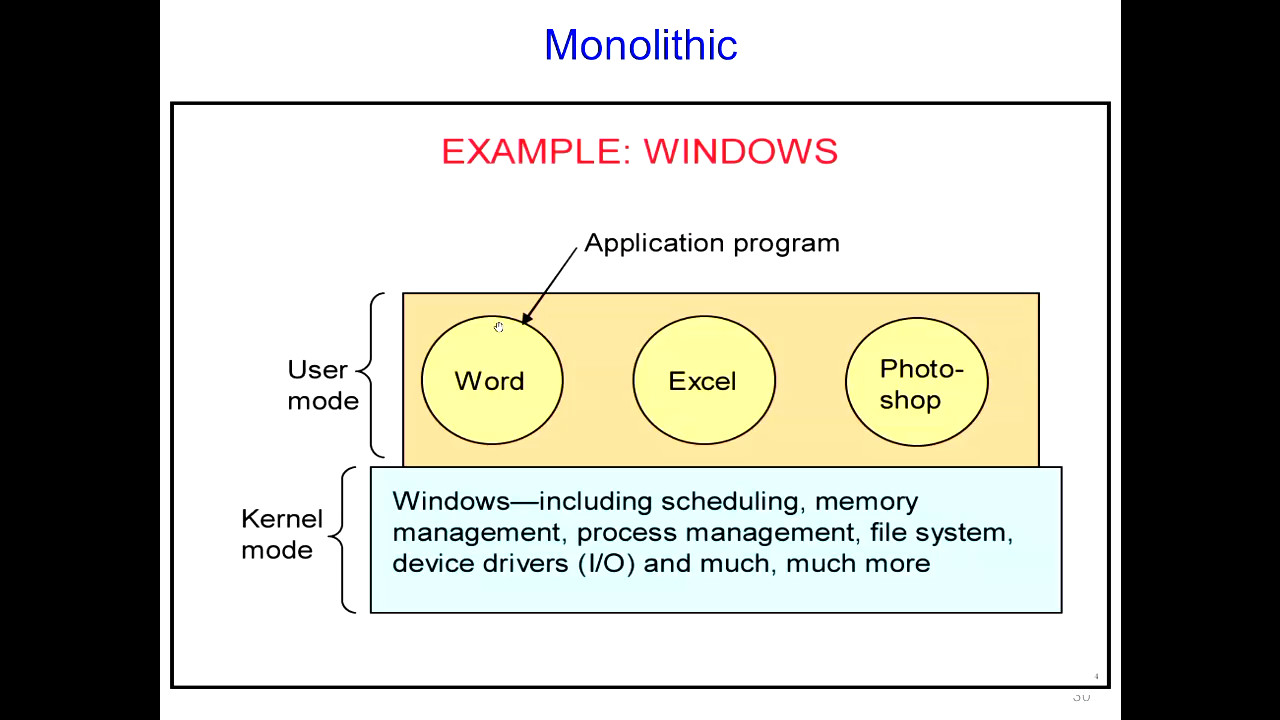
\includegraphics[height=270]{windows}

MINIX 3

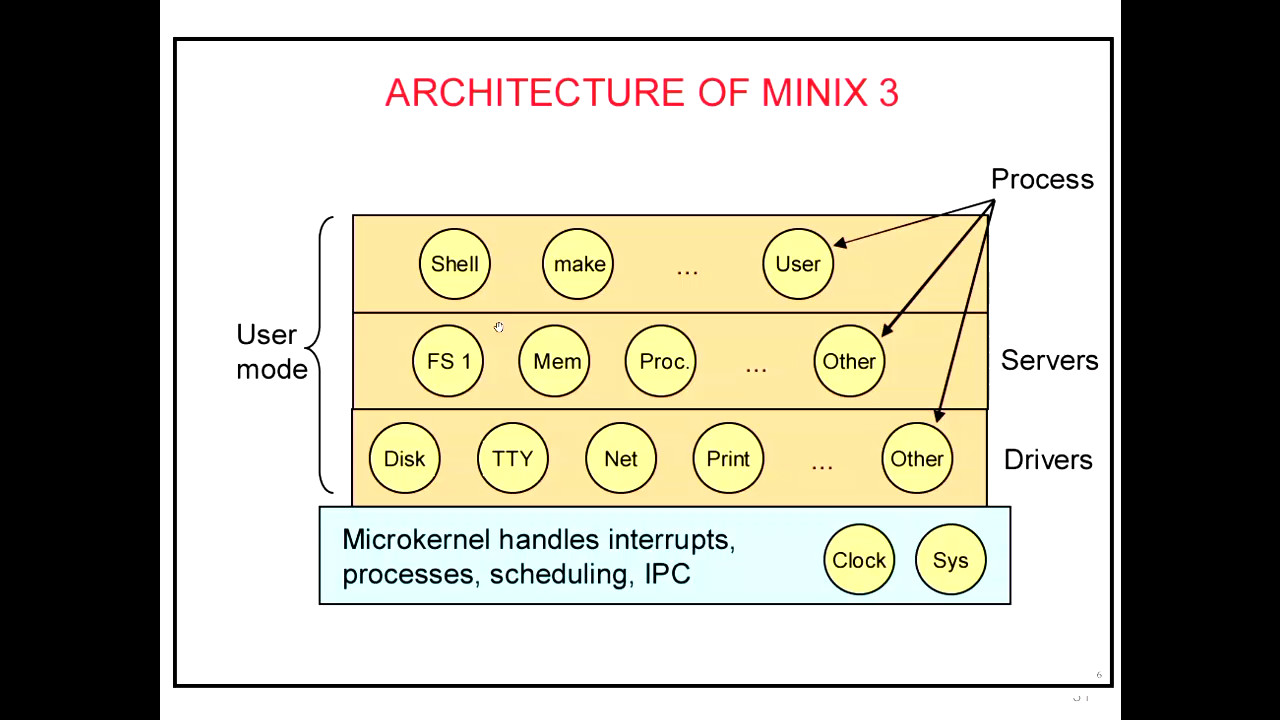
\includegraphics[height=270]{minix-3}

\subsection{Loadable kernel modules}

\begin{itemize}
    \item (Perhaps) the best practice for OS design
    \item Core services in the kernel, and others dynamically loaded
    \item Common implementations include: Solaris, Linux, etc.
    \item Advantages
        \begin{itemize}
            \item convenient: no need for rebooting for newly added modules
            \item efficient: no need for message passing unlike micro-kernel
            \item flexible: any module can call any other module unlike layered model
        \end{itemize}
\end{itemize}

\subsection{Summary}

\begin{itemize}
    \item Fundamental distinction between user and privileged mode supported by most hardware
    \item OS design has been an evolutionary process of trial and error.
    \item Successful OS designs have run the spectrum  from monolithic, to layered,
        to micro-kernels
    \item The role and design of an OS are still evolving
    \item It is impossible to pick one ``correct'' way to structure an OS
\end{itemize}

\section{Lecture 3: Processes}

\subsection{What is a ``process''?}

\begin{itemize}
    \item The process is the OS\emph{s} abstraction for execution
        \begin{itemize}
            \item A process is a program in execution
        \end{itemize}
    \item Simplest (classic) case: a \emph{sequential process}
        \begin{itemize}
            \item An address space (an abstraction of memory)
            \item A single thread of execution (an abstraction of the CPU)
        \end{itemize}
    \item A sequential process is:
        \begin{itemize}
            \item The unit of execution
            \item The unit of scheduling
            \item The dynamic (active) execution context
                (as opposed to the program --- static, just a bunch of bytes)
        \end{itemize}

\end{itemize}

\subsection{What's ``in'' a process?}

\begin{itemize}
    \item A process consists of (at least):
        \begin{itemize}
            \item An \emph{address space}, containing:
                \begin{itemize}
                    \item the code (instructions) for the running program
                    \item the data for the running program (static data, heap data, stack)
                \end{itemize}
            \item \emph{CPU state}, consisting of:
                \begin{itemize}
                    \item the program counter (PC), indicating the next instruction;
                    \item the stack pointer;
                    \item other general purpose register values.
                \end{itemize}
            \item A set of \emph{OS resources}
                \begin{itemize}
                    \item open files, network connections, sound channels, \dots
                \end{itemize}
            \item In other words, everything needed to run the program
                (or to restart, if interrupted).
        \end{itemize}
\end{itemize}

\begin{center}{}
    \includegraphics[height=280]{a-process's-address-space}
\end{center}

\subsection{The OS process namespace}

\begin{itemize}
    \item The particulars depend on the specific OS, but the principles are general;
    \item The name for a process is called a \emph{process ID} (PID) (an integer);
    \item The PID namespace is global to the system;
    \item Operations that create processes return a PID (e.g.\ fork);
    \item Operations on processes take PIDs as an argument (e.g.\ kill, wait, nice).\
\end{itemize}

\subsection{Representation of processes by the OS}

\begin{itemize}
    \item The OS maintains a data structure to keep track of a process's state
        \begin{itemize}
            \item called the \emph{process control block} (PCB)
                or \emph{process descriptor};
            \item identified by the PID.\
        \end{itemize}
    \item OS keeps all of a process's execution state in (or linked from) the PCB
        when the process isn't running
        \begin{itemize}
            \item PC, SP, registers, etc.
            \item when a process is unscheduled, the state is transferred out of the
                hardware into the PCB
            \item (when a process is running, its state is spread between the PCB and the CPU).
        \end{itemize}
\end{itemize}

\subsection{The PCB}

\begin{itemize}
    \item The PCB is a data structure with many, many fields
    \begin{itemize}
        \item PID
        \item parent PID
        \item execution state
        \item PC, SP, registers
        \item address space info
        \item UNIX user id, group id
        \item scheduling priority
        \item accounting info
        \item pointers for state queues
    \end{itemize}
\item In Linux:
    \begin{itemize}
        \item defined in \texttt{task\_struct (include/linux/sched.h)}
        \item Over 95 fields!
    \end{itemize}<++>
\end{itemize}<++>

\end{document}
